\part{Dissipative-particle-dynamics model for two-phase flows}
\frame{\partpage}

\section{两相的DPD模型}
\frame{\frametitle{DPD与分子动力学的差别}

\begin{columns}
\begin{column}[c]{0.5\textwidth}
\begin{center}
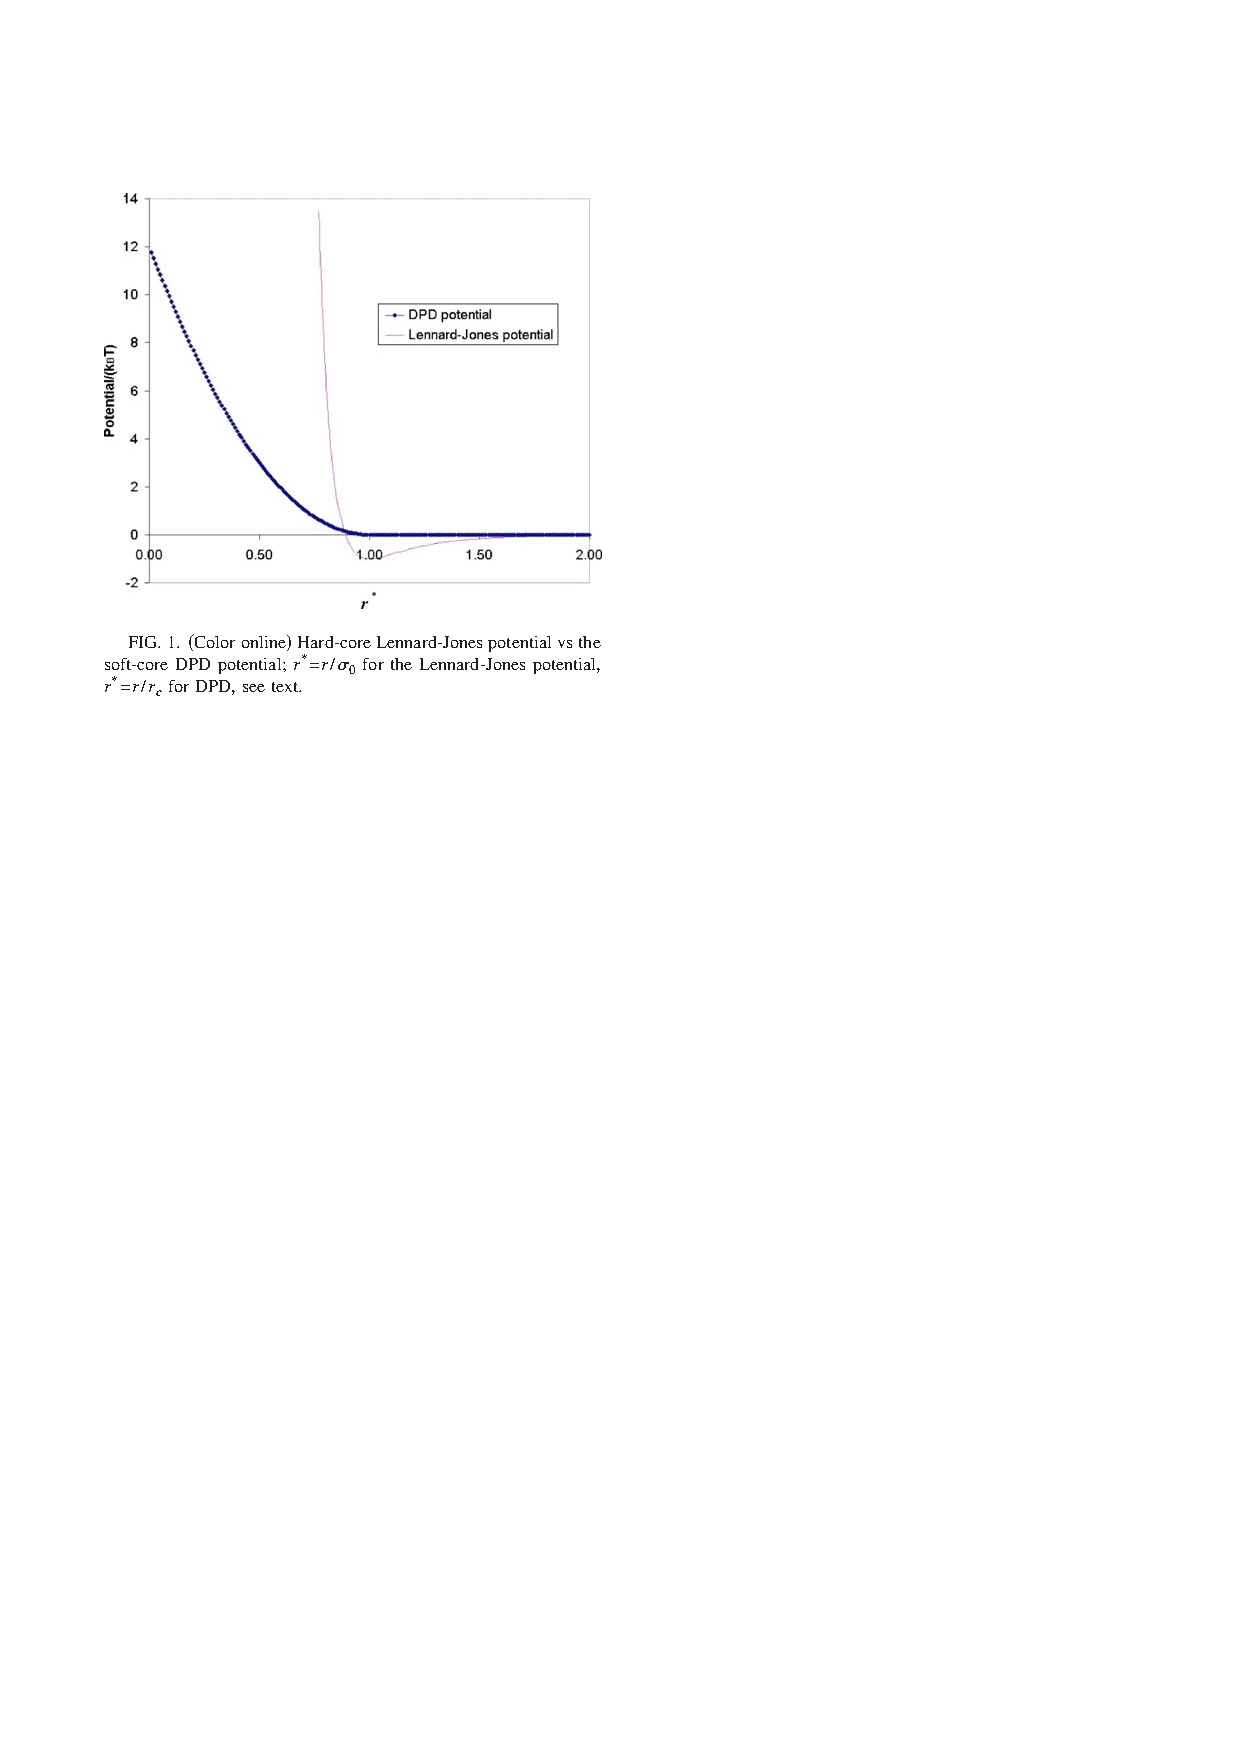
\includegraphics[width=\textwidth]{./figures/PotentialVsR.pdf}
\end{center}
\end{column}
\begin{column}[c]{0.5\textwidth}
\begin{enumerate}
\item lennard-Jones 势能的斜率太陡,力的变化太快,因此对$\Delta t$的要求较高。
\item DPD 势能的斜率相对lennard-Jones 势能比较平缓。对应的守恒力
\[F_{ij}^C=a_{ij}(1-r_{ij}/r_c)e_{ij}\]
\end{enumerate}
\end{column}
\end{columns}
}

\frame{\frametitle{van der waals 状态方程}
\begin{columns}
\begin{column}[c]{0.5\textwidth}
\begin{center}
\includegraphics[width=\textwidth]<2->{./figures/van_der_Walls.pdf}
\end{center}
\end{column}
\begin{column}[c]{0.5\textwidth}
\begin{enumerate}
%\item<1-> 保守力可由自由导出:$\mathbf{F}_{ij}^C = - \frac{\partial \psi(r_{ij})}{\partial r_{ij}}\mathbf{e_{ij}}$
\item<1-> 耗散力和随机力反应流体力学的性质, 保守力表现热力学的性质。
\item<3-> 保守力\\$F_{ij}^C=a_{ij}(1-r_{ij}/r_c)e_{ij}$\\
  并不能体现表现表面张力的长程力。
 \item<4-> 能引起相分离和表面张力的保守力形式\\
 $F^C=-\nabla \psi_{nonideal}+F^S$
\end{enumerate}
\end{column}
\end{columns}
}

\frame{\frametitle{平均自由能及其泰勒展开}

每个粒子的平均自由能
\begin{equation}
\psi_m = \int u_{att}(r)\rho dr\ \  \underrightarrow{\textrm{泰勒展开}}
\ \ \psi_m = -a\rho - k\nabla^2\rho
\end{equation}

其中

\[
a = -\frac{1}{2}\int_{r>\sigma_0}u_{att}(r)dr, \ \ \ \kappa = -\frac{1}{6}\int_{r>\sigma_0}r^2u_{att}(r)dr
\]

}

\frame{\frametitle{基于van der waals 状态方程的自由能}

由van der waals 状态方程
\[
(p+\frac{n^2a}{V^2})(V-nb)=nRT \Longrightarrow p = \frac{\rho k_B T}{1-b\rho}-a\rho^2
\]

结合$p=\frac{\partial \psi}{\partial v}$ 可得

\begin{center}
$\psi = \underline{\textcolor{red}{-k_bT\ln(1-b\rho)-a\rho}}+\underline{\textcolor{blue}{k_BT\ln\rho}}$\\
\ \ \ \ \ \ \ \ \ \ $\textcolor{red}{\psi_{non-ideal}}$ \ \ \ \ \ \ \ \ \ \ \ \ \ \ \ $\textcolor{blue}{F^S}$
\end{center}
}

\frame{\frametitle{密度的计算}

密度的计算采用了SPH中密度计算的方法
\[
\rho_i=\sum_{j=1}^N w(r_{ij})
\]

其中$w$满足: $ \int_0^{r_{c}}2\pi rw(r)rdr = 1$, 二维的权函数$w$如下

\begin{displaymath}
w(r,r_C) = \left\{\begin{array}{ll}
\frac{5}{\pi r_C^2}(1+\frac{3r}{r_c})(1-\frac{r}{r_C})^3 & \textrm{if $r<r_c$}\\
0 & \textrm{if $r>r_c$}
\end{array} \right.
\end{displaymath}
}

\frame{\frametitle{保守力的最终表达式}

表面张力项

\[
F^S=\kappa \nabla\nabla^2\rho
\]

因此保守力为

\[
F^C=\nabla[k_bT\ln(1-b\rho)+a\rho]+\kappa\nabla\nabla^2\rho
\]

结合前面相关结果,最终得到

\[
f_{ij}^C=\Big[-\Big\{\big(\frac{bk_BT}{1-b\rho_i}\big)+\big(\frac{bk_BT}{1-b\rho_j}-a\big)\Big\}w_{ij}^{(1)}+\kappa w_{ij}^{(3)}\Big]
\]
}

\section{算例}
\subsection{Liquid layer simulations}

\frame{\frametitle{结构与参数}
\begin{columns}
\begin{column}[c]{0.5\textwidth}
\begin{center}
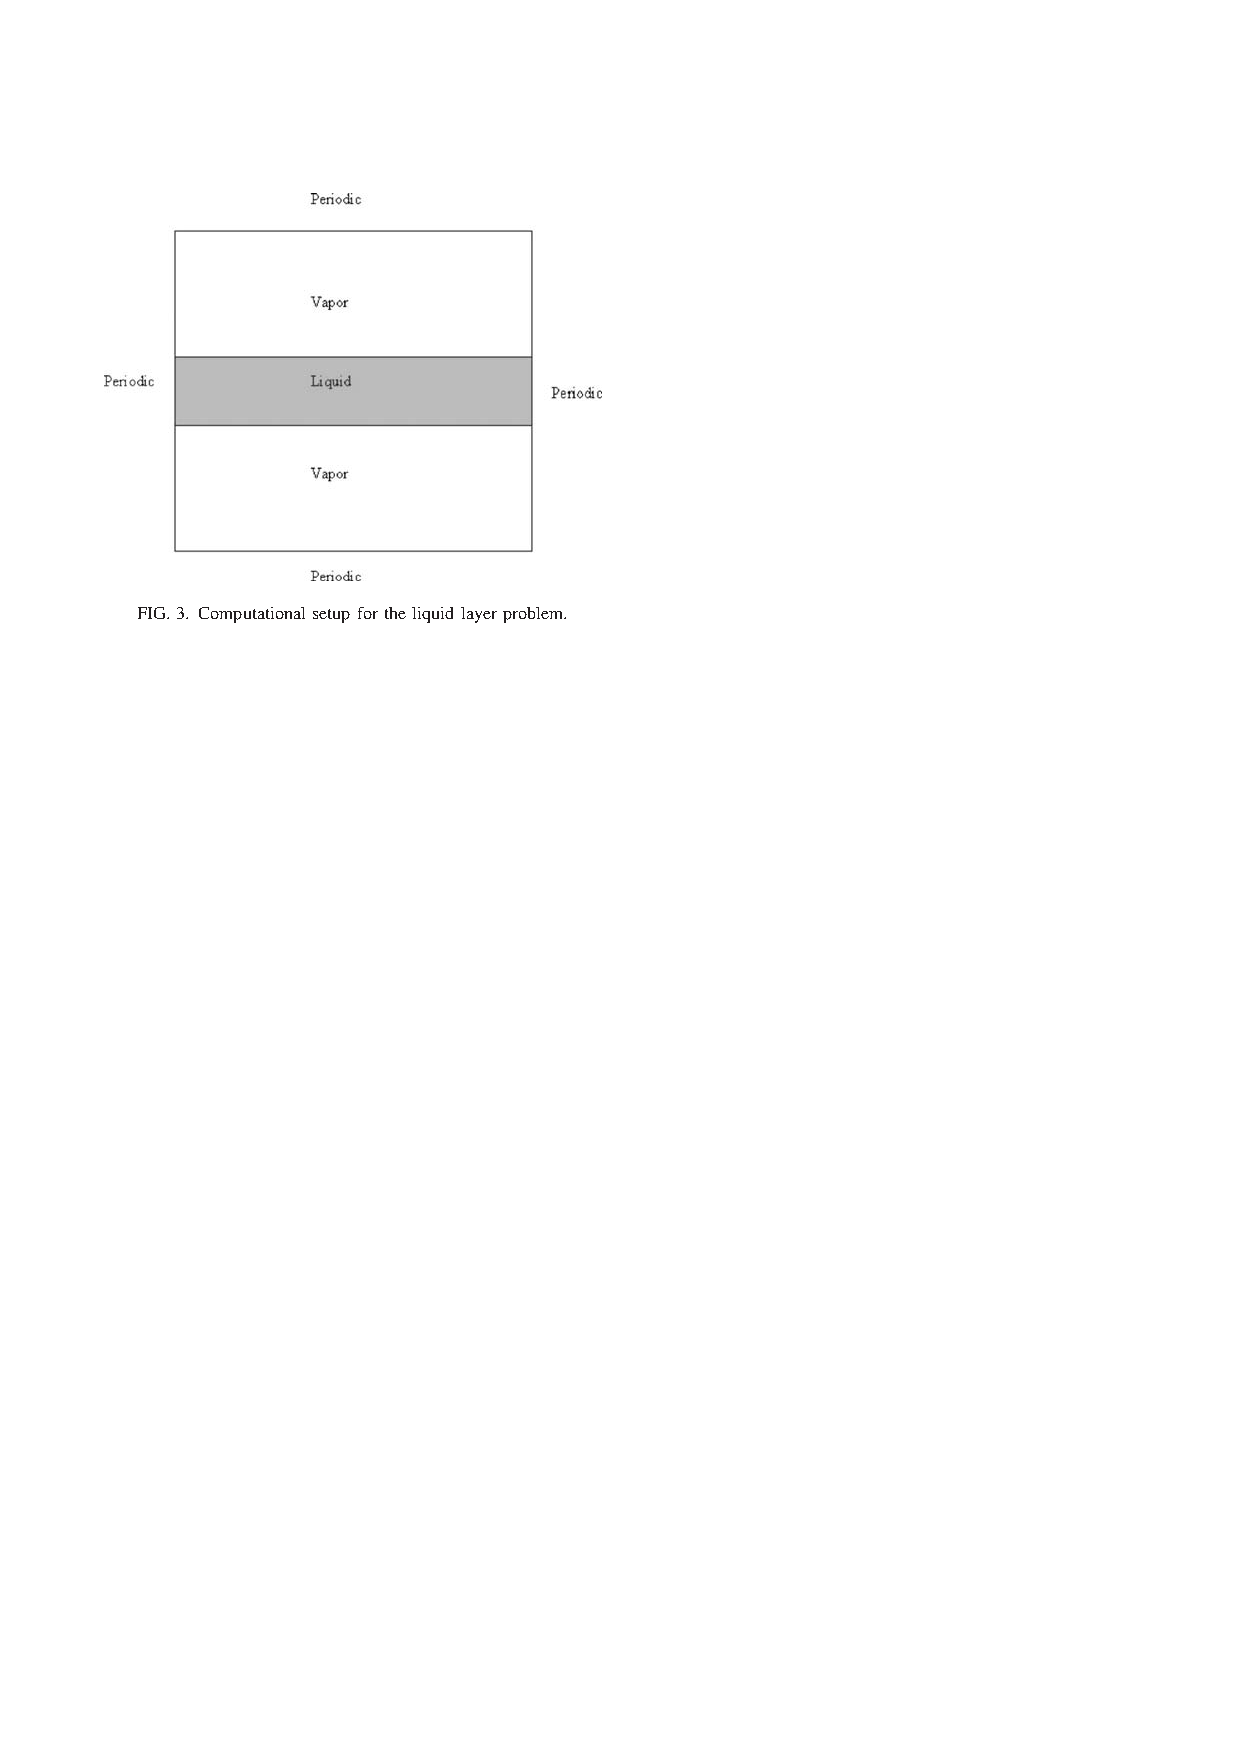
\includegraphics[width=1\textwidth]{./figures/configuration.pdf}
\end{center}
\end{column}
\begin{column}[c]{0.5\textwidth}
\begin{center}
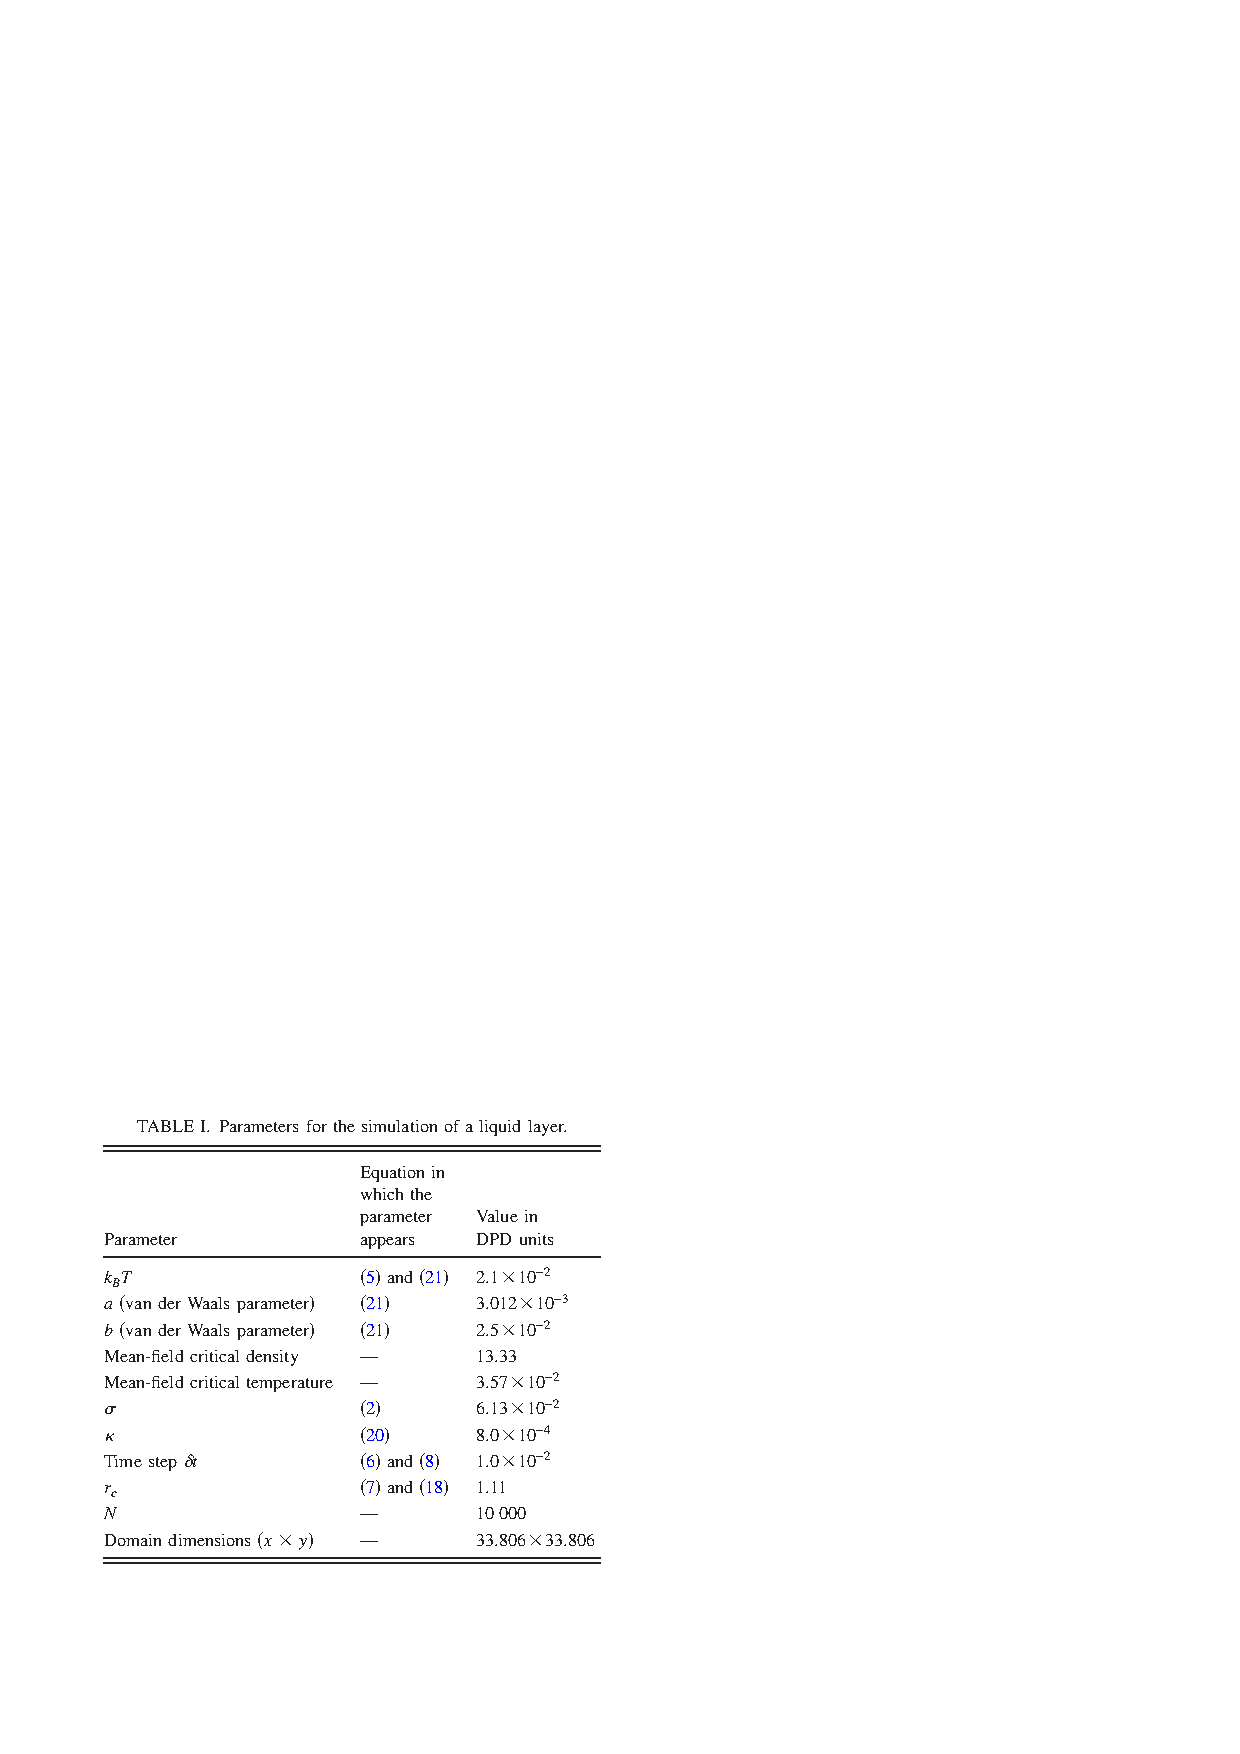
\includegraphics[width=1\textwidth]{./figures/parameter.pdf}
\end{center}
\end{column}
\end{columns}
}

\frame{\frametitle{表面张力的计算}
\begin{columns}
\begin{column}[c]{0.5\textwidth}
\begin{center}
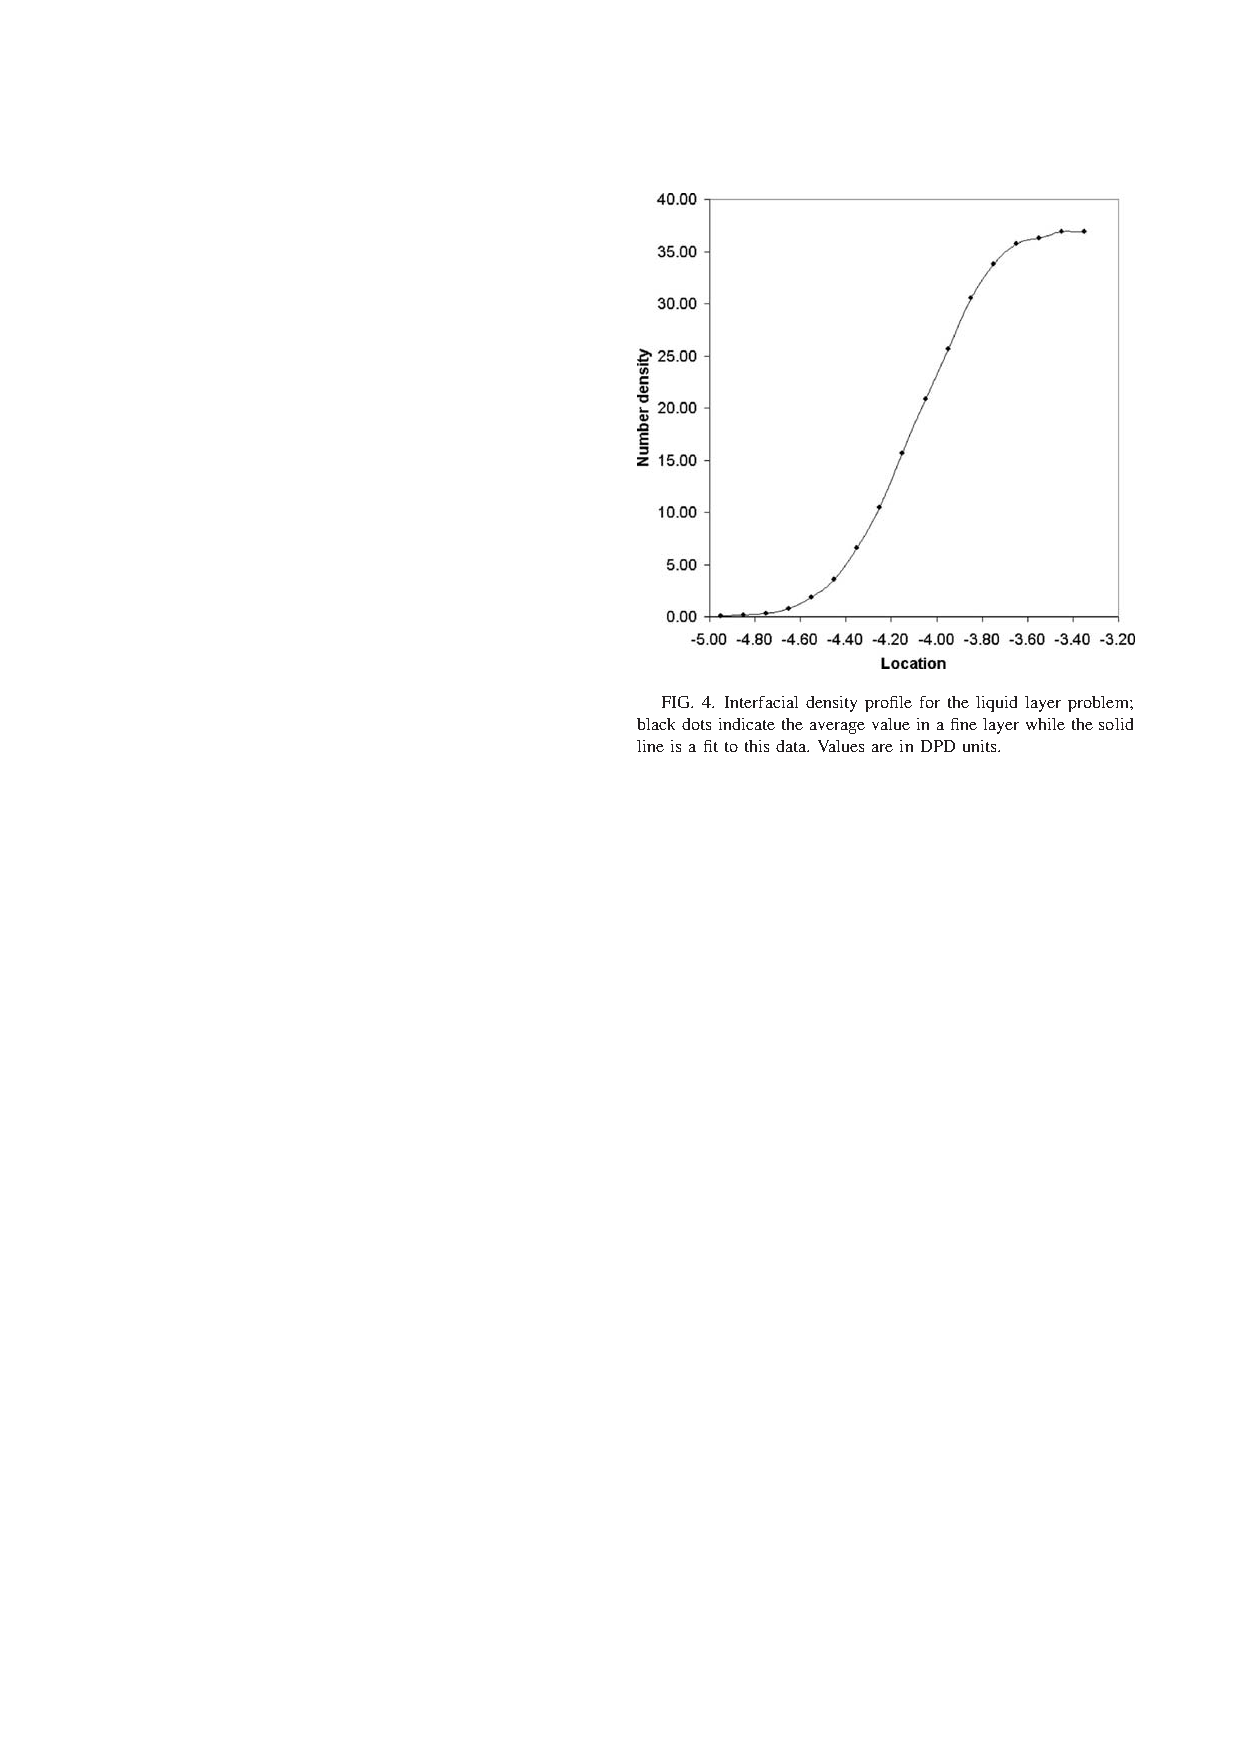
\includegraphics[width=1\textwidth]{./figures/density.pdf}
\end{center}
\end{column}
\begin{column}[c]{0.5\textwidth}
表面张力计算公式:
\[
\sigma_s=\kappa \int_{-\infty}^{+\infty}\Big(\frac{\partial \rho}{\partial n}\Big)dn
\]
\end{column}
\end{columns}
}

\subsection{Laplace law simulations}

\frame{\frametitle{结构与计算方法}
\begin{columns}
\begin{column}[c]{0.5\textwidth}
\begin{center}
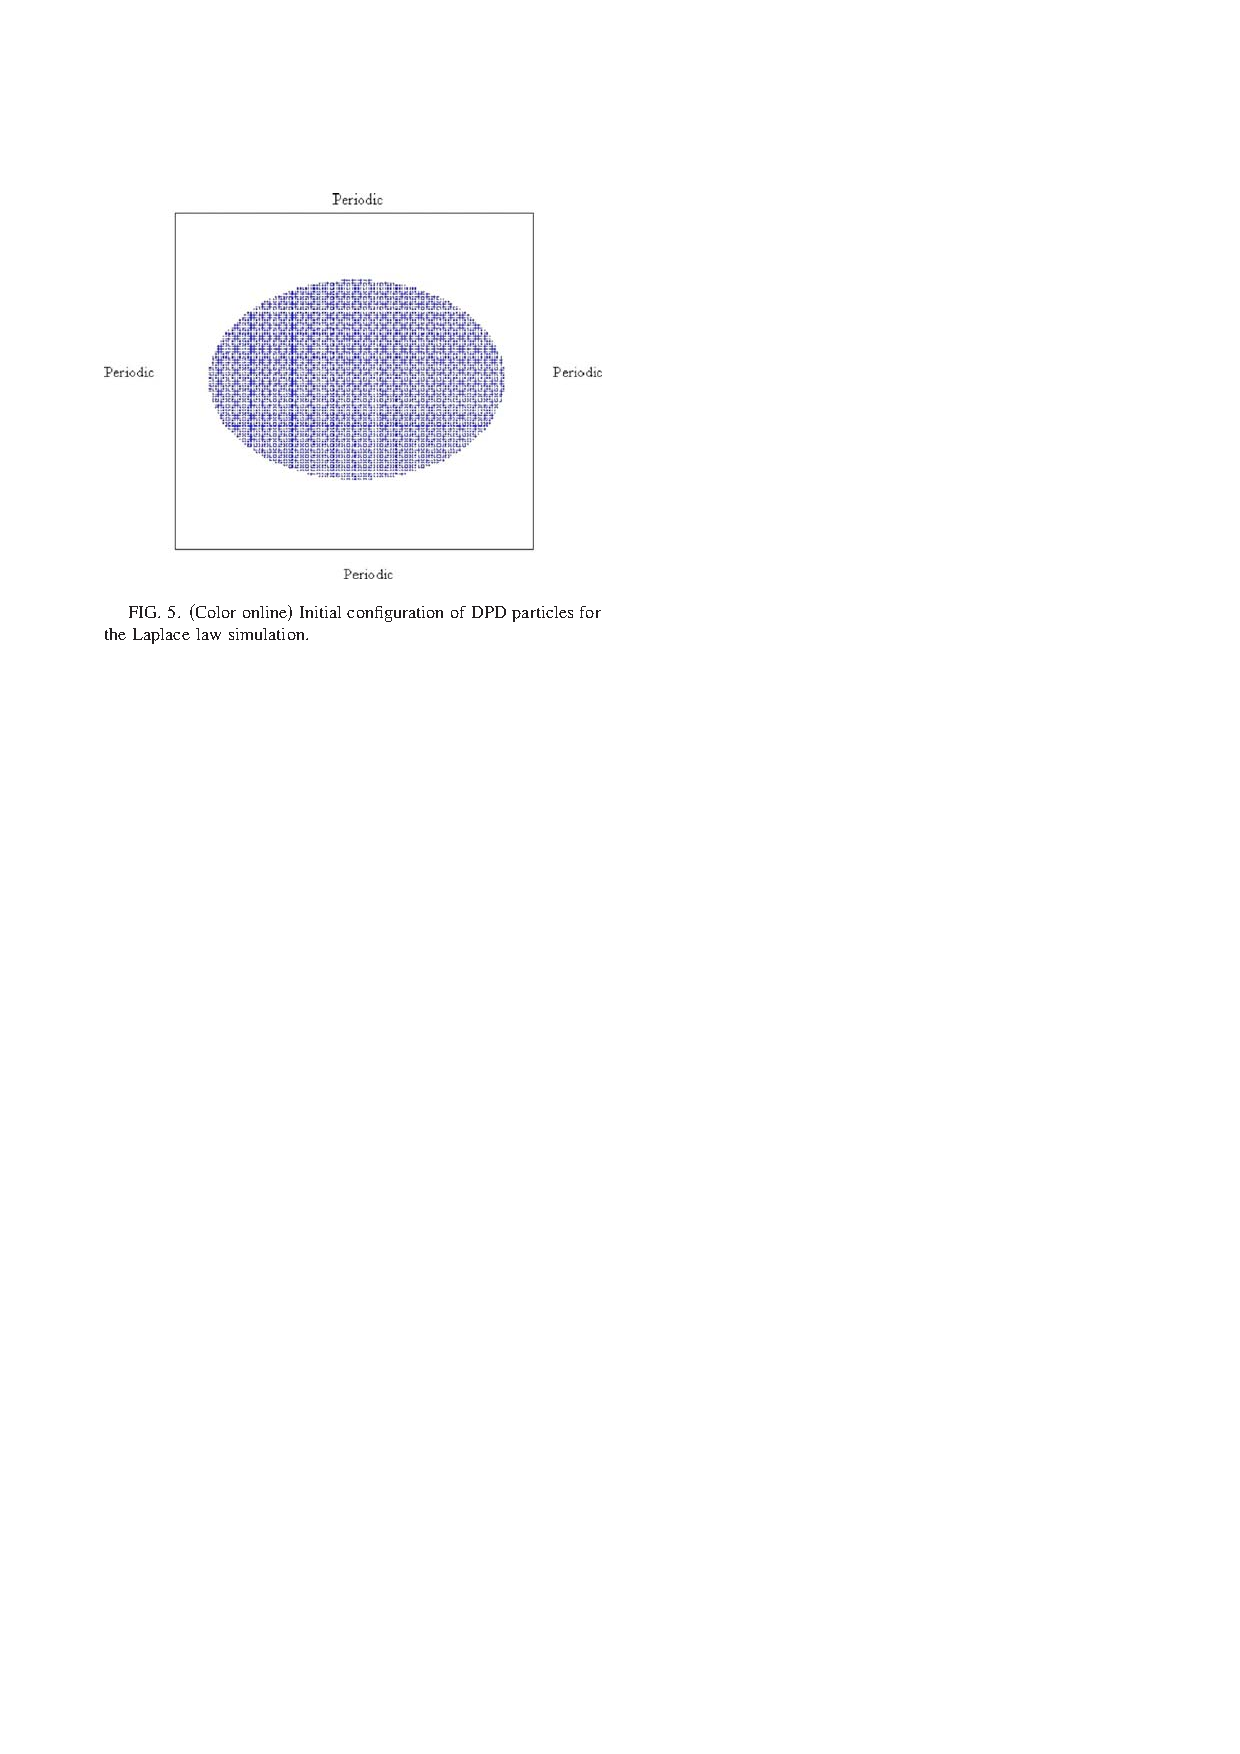
\includegraphics[width=1\textwidth]{./figures/configuration2.pdf}
\end{center}
\end{column}
\begin{column}[c]{0.5\textwidth}
二维的Laplace law 如下:
\[
p_{in}-p_{out}=\frac{\sigma_s}{R}
\]
压强和曲率半径的计算:
\[
p=\rho k_BT+\frac{1}{2dV}\sum_i\sum_jr_{ij}F_{ij}^C
\]

\[
R=\sqrt{N/(\pi\rho_{eq})}
\]
\end{column}
\end{columns}
}

\frame{\frametitle{Laplace law的证明}
\begin{center}
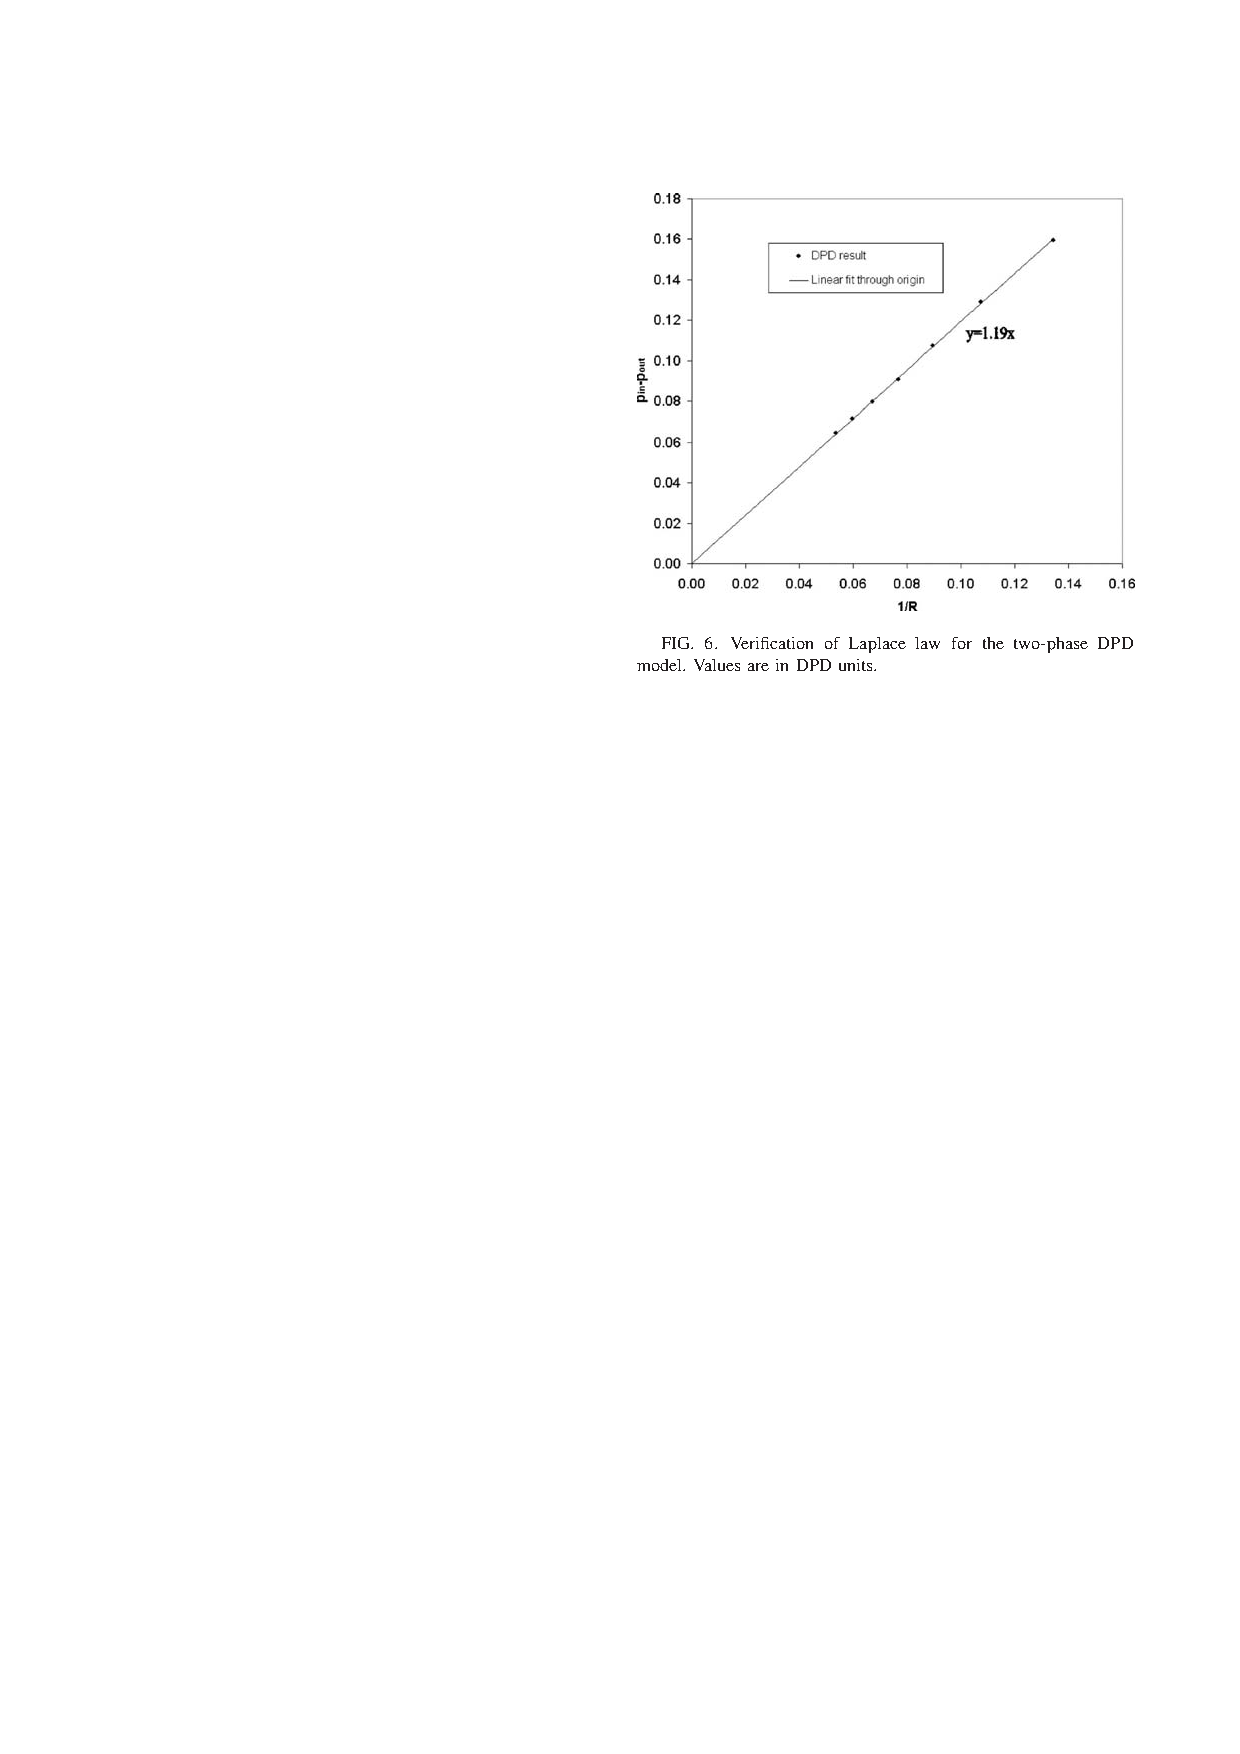
\includegraphics[width=0.6\textwidth]{./figures/verificationLaplace.pdf}
\end{center}
}

\subsection{Ocillation of a liquid cylinder}

\frame{\frametitle{Small-amplitude oscillations}
\begin{columns}
\begin{column}[c]{0.5\textwidth}
\begin{center}
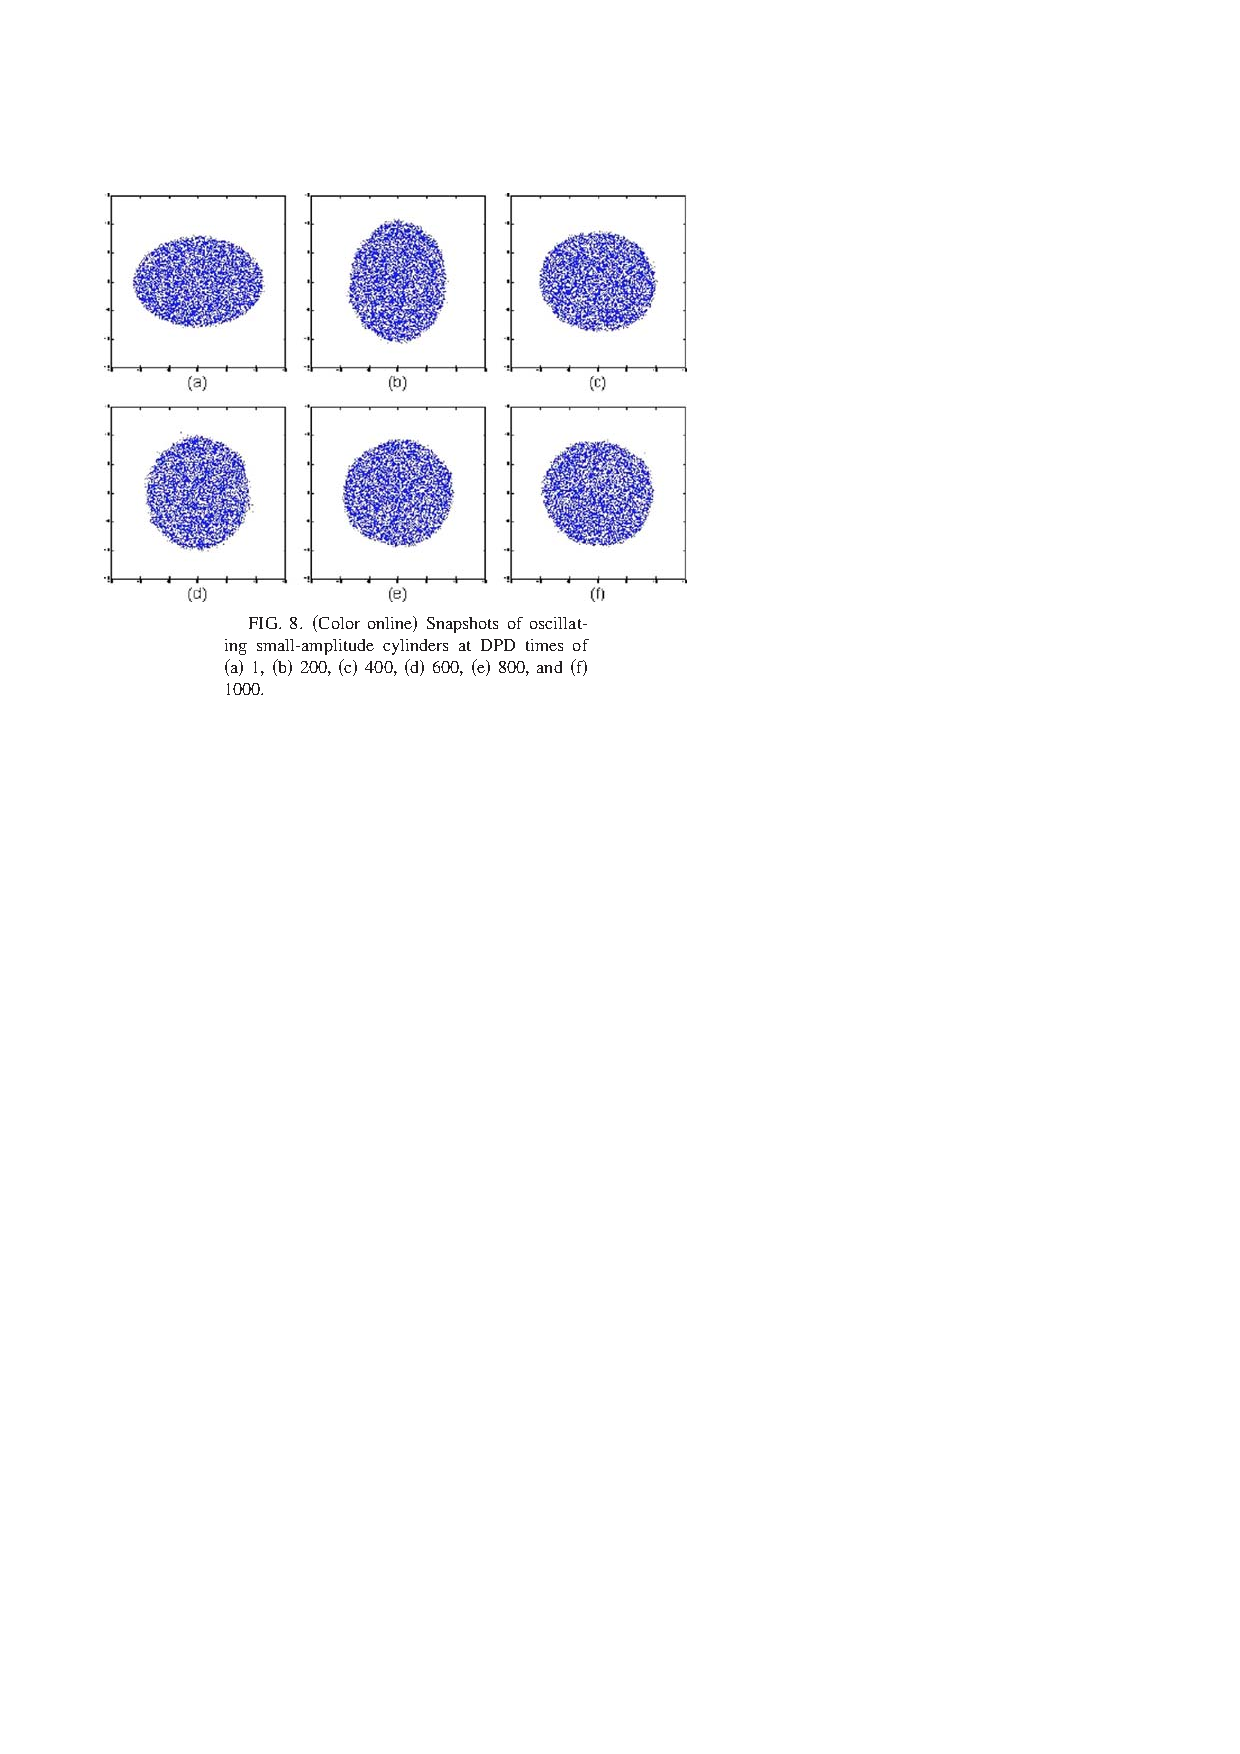
\includegraphics[width=1\textwidth]{./figures/oscillate.pdf}
\end{center}
\end{column}
\begin{column}[c]{0.5\textwidth}
\begin{center}
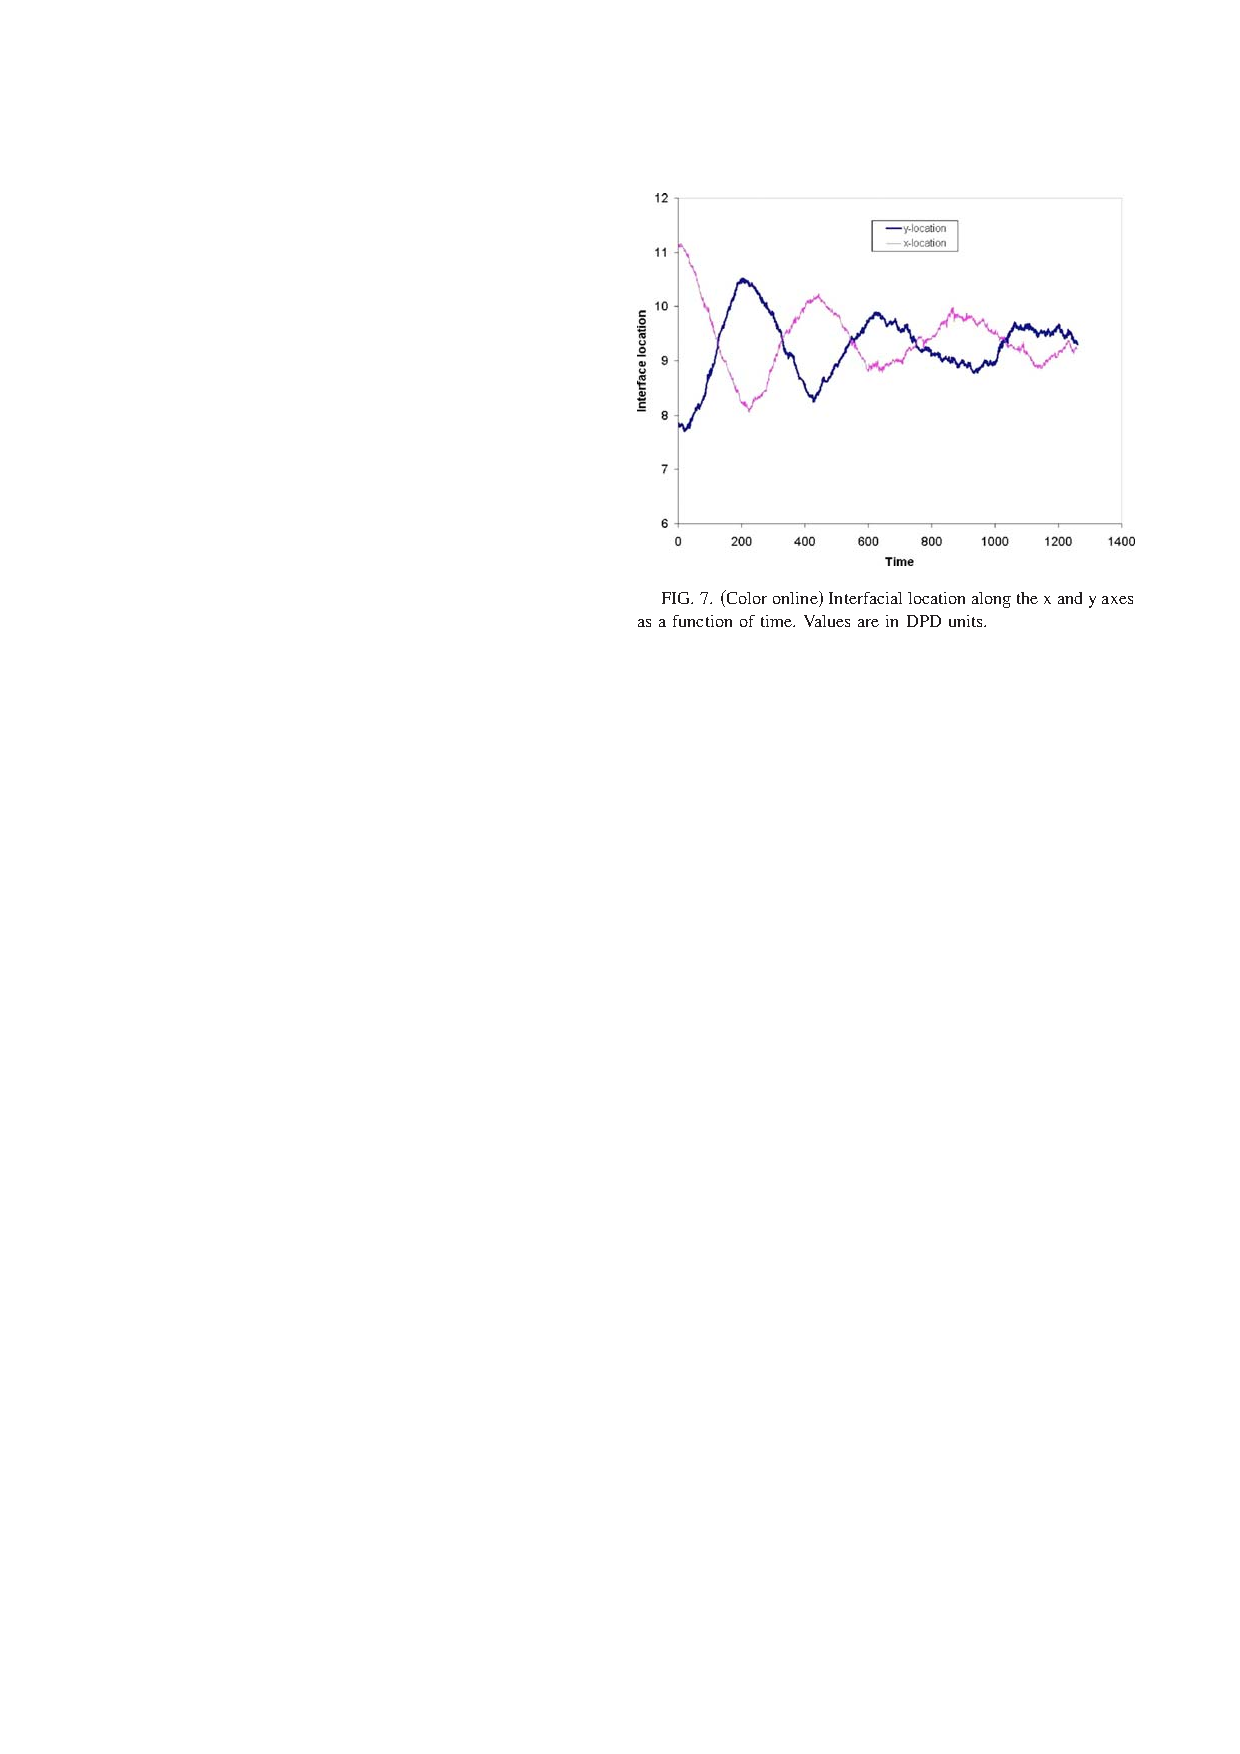
\includegraphics[width=1\textwidth]{./figures/InterfaceLocation.pdf}
\end{center}
\end{column}
\end{columns}
}

\frame{\frametitle{Large-amplitude oscillations}

\begin{center}
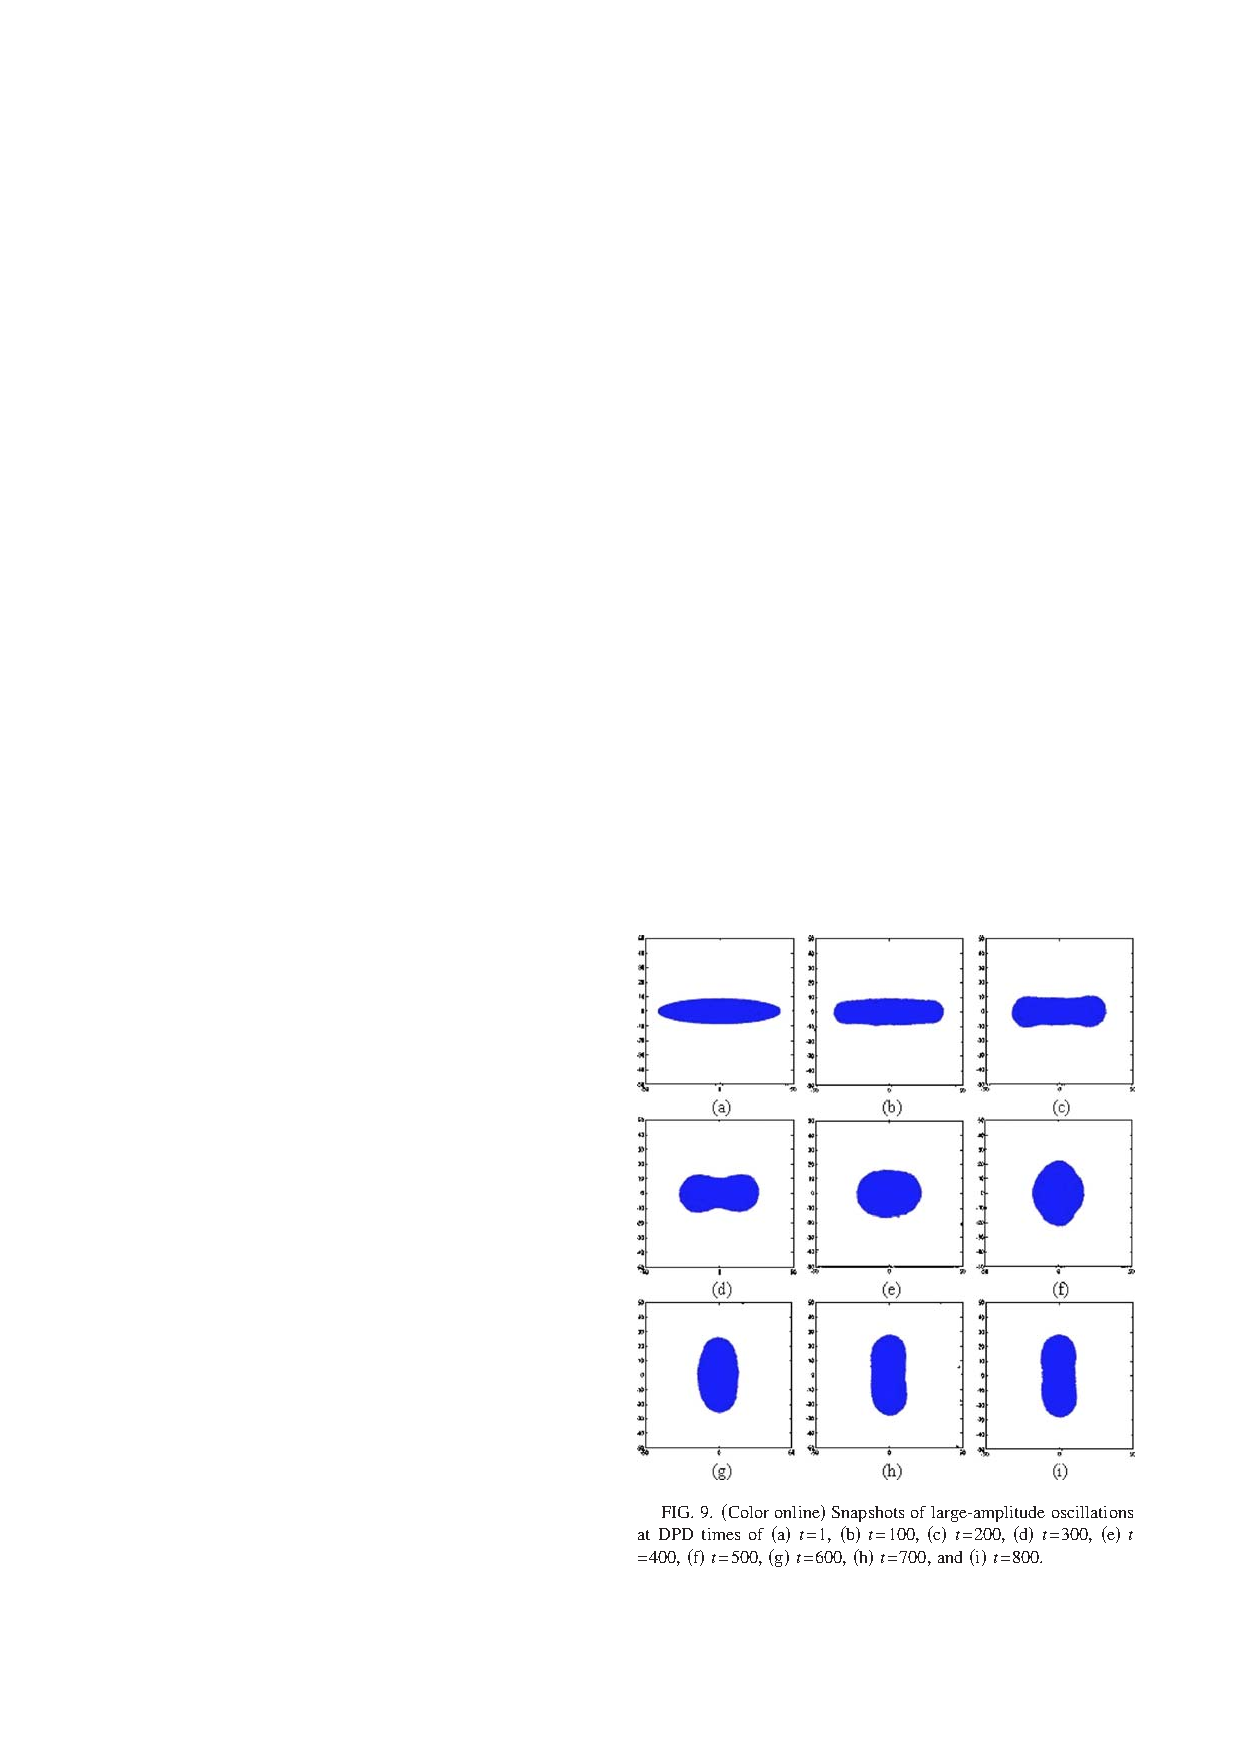
\includegraphics[width=0.5\textwidth]{./figures/LargeAmplitude.pdf}
\end{center}
}

